\documentclass[twoside]{book}

% Packages required by doxygen
\usepackage{fixltx2e}
\usepackage{calc}
\usepackage{doxygen}
\usepackage[export]{adjustbox} % also loads graphicx
\usepackage{graphicx}
\usepackage[utf8]{inputenc}
\usepackage{makeidx}
\usepackage{multicol}
\usepackage{multirow}
\PassOptionsToPackage{warn}{textcomp}
\usepackage{textcomp}
\usepackage[nointegrals]{wasysym}
\usepackage[table]{xcolor}

% Font selection
\usepackage[T1]{fontenc}
\usepackage[scaled=.90]{helvet}
\usepackage{courier}
\usepackage{amssymb}
\usepackage{sectsty}
\renewcommand{\familydefault}{\sfdefault}
\allsectionsfont{%
  \fontseries{bc}\selectfont%
  \color{darkgray}%
}
\renewcommand{\DoxyLabelFont}{%
  \fontseries{bc}\selectfont%
  \color{darkgray}%
}
\newcommand{\+}{\discretionary{\mbox{\scriptsize$\hookleftarrow$}}{}{}}

% Page & text layout
\usepackage{geometry}
\geometry{%
  a4paper,%
  top=2.5cm,%
  bottom=2.5cm,%
  left=2.5cm,%
  right=2.5cm%
}
\tolerance=750
\hfuzz=15pt
\hbadness=750
\setlength{\emergencystretch}{15pt}
\setlength{\parindent}{0cm}
\setlength{\parskip}{3ex plus 2ex minus 2ex}
\makeatletter
\renewcommand{\paragraph}{%
  \@startsection{paragraph}{4}{0ex}{-1.0ex}{1.0ex}{%
    \normalfont\normalsize\bfseries\SS@parafont%
  }%
}
\renewcommand{\subparagraph}{%
  \@startsection{subparagraph}{5}{0ex}{-1.0ex}{1.0ex}{%
    \normalfont\normalsize\bfseries\SS@subparafont%
  }%
}
\makeatother

% Headers & footers
\usepackage{fancyhdr}
\pagestyle{fancyplain}
\fancyhead[LE]{\fancyplain{}{\bfseries\thepage}}
\fancyhead[CE]{\fancyplain{}{}}
\fancyhead[RE]{\fancyplain{}{\bfseries\leftmark}}
\fancyhead[LO]{\fancyplain{}{\bfseries\rightmark}}
\fancyhead[CO]{\fancyplain{}{}}
\fancyhead[RO]{\fancyplain{}{\bfseries\thepage}}
\fancyfoot[LE]{\fancyplain{}{}}
\fancyfoot[CE]{\fancyplain{}{}}
\fancyfoot[RE]{\fancyplain{}{\bfseries\scriptsize Generated by Doxygen }}
\fancyfoot[LO]{\fancyplain{}{\bfseries\scriptsize Generated by Doxygen }}
\fancyfoot[CO]{\fancyplain{}{}}
\fancyfoot[RO]{\fancyplain{}{}}
\renewcommand{\footrulewidth}{0.4pt}
\renewcommand{\chaptermark}[1]{%
  \markboth{#1}{}%
}
\renewcommand{\sectionmark}[1]{%
  \markright{\thesection\ #1}%
}

% Indices & bibliography
\usepackage{natbib}
\usepackage[titles]{tocloft}
\setcounter{tocdepth}{3}
\setcounter{secnumdepth}{5}
\makeindex

% Hyperlinks (required, but should be loaded last)
\usepackage{ifpdf}
\ifpdf
  \usepackage[pdftex,pagebackref=true]{hyperref}
\else
  \usepackage[ps2pdf,pagebackref=true]{hyperref}
\fi
\hypersetup{%
  colorlinks=true,%
  linkcolor=blue,%
  citecolor=blue,%
  unicode%
}

% Custom commands
\newcommand{\clearemptydoublepage}{%
  \newpage{\pagestyle{empty}\cleardoublepage}%
}

\usepackage{caption}
\captionsetup{labelsep=space,justification=centering,font={bf},singlelinecheck=off,skip=4pt,position=top}

%===== C O N T E N T S =====

\begin{document}

% Titlepage & ToC
\hypersetup{pageanchor=false,
             bookmarksnumbered=true,
             pdfencoding=unicode
            }
\pagenumbering{alph}
\begin{titlepage}
\vspace*{7cm}
\begin{center}%
{\Large Grasp Planner }\\
\vspace*{1cm}
{\large Generated by Doxygen 1.8.13}\\
\end{center}
\end{titlepage}
\clearemptydoublepage
\pagenumbering{roman}
\tableofcontents
\clearemptydoublepage
\pagenumbering{arabic}
\hypersetup{pageanchor=true}

%--- Begin generated contents ---
\chapter{Main Page}
\label{index}\hypertarget{index}{}\subsubsection*{This R\+O\+S2 package provides an {\bfseries algorithmic, depth based approach} to generate a {\bfseries 3+1 Degree of Freedom (D\+OF) Grasp pose} from a depth image.}

\href{https://travis-ci.com/gtan039/algorithmic-depth-based-grasp-planner}{\tt }

\section*{Introduction}

Traditionally, grasp pose generation is done through using convolutional neural networks (C\+N\+Ns) to achieve grasp plans. The issues with using machine learning and neural networks is several fold


\begin{DoxyEnumerate}
\item Computation power required for fast grasp pose planning using C\+N\+Ns.
\item Dataset for training neural netwoks are currently restricted to 2 finger grippers (notably, the \href{http://pr.cs.cornell.edu/grasping/rect_data/data.php}{\tt Cornell Grasping Dataset} has been the most comprehensive and well labelled dataset for current grasp planning neural networks)
\item Training of new types of grippers require {\bfseries manual labelling} of new datasets (labour intensive).
\item Accurate and stable grasp poses may not be available for {\bfseries irregular objects}, so specifically labelled dataset is needed in order to generate accurate grasps
\end{DoxyEnumerate}

\subsection*{Package example}

This R\+O\+S2 package presents a solution that requires no training, no labelling and little computational power to generate a 3 + 1 D\+OF grasp poses. The modular design of this package also allows for expansion into other gripper types. Current support for this package includes {\bfseries 2 finger gripper and single suction cup gripper}

~\newline


\section*{Package Details}

\subsection*{Assumptions}

\subsubsection*{Grasp object poses}

This package assumes a {\bfseries top down} camera set up overlooking the grasping area. Assuming that the axis through the image plane is the z axis, grasp poses will consider a {\bfseries one dimensional change in orientation} in the z-\/direction (resulting in a 3+1 D\+OF grasp pose)

\subsubsection*{Image Quality}

This package was tested using an input depth image from the Intel Realsense D415 R\+G\+B-\/D camera. Certain variations may occur if a different camera is used

\subsubsection*{Work Surface}

This package assumes that the object is placed on a relatively flat surface. As this package requires the use of the depth image from the camera above the work surface, we assume that the distance from the work surface to the camera is constant.

\subsubsection*{End Effector Support}

This package currently supports a 2 Finger gripper and a single suction cup gripper. Further development will include multiple finger gripper and suction cup array support.

\subsection*{Package subscriber}

This package consists of a subscriber that subscribes to the following topic with the message structure shown

Topic Name \+: {\ttfamily /perception\+\_\+output}

Message Name\+: Rect\+Output.\+msg

\tabulinesep=1mm
\begin{longtabu} spread 0pt [c]{*{3}{|X[-1]}|}
\hline
\rowcolor{\tableheadbgcolor}\textbf{ Message name }&\textbf{ Field Type }&\textbf{ Explanation  }\\\cline{1-3}
\endfirsthead
\hline
\endfoot
\hline
\rowcolor{\tableheadbgcolor}\textbf{ Message name }&\textbf{ Field Type }&\textbf{ Explanation  }\\\cline{1-3}
\endhead
header &std\+\_\+msgs/\+Header &General information from the camera \\\cline{1-3}
objects &Dl\+Object\mbox{[}\mbox{]} &Information about the object (refer below to the Dl\+O\+Bject message type. \\\cline{1-3}
frame\+\_\+width &uint32 &Width of the depth image \\\cline{1-3}
frame\+\_\+height &uint32 &Height of the depth image \\\cline{1-3}
num\+\_\+objects &uint32 &Number of objects in scene \\\cline{1-3}
depth\+\_\+image &sensor\+\_\+msgs/\+Image &Depth image of the work area \\\cline{1-3}
camera\+\_\+info &sensor\+\_\+msgs/\+Camera\+Info &Camera-\/specific information \\\cline{1-3}
roi\+\_\+array &sensor\+\_\+msgs/\+Region\+Of\+Interest\mbox{[}\mbox{]} &Array of bounding boxes containing the objects \\\cline{1-3}
\end{longtabu}
Message Name\+: Dl\+Object.\+msg

\tabulinesep=1mm
\begin{longtabu} spread 0pt [c]{*{3}{|X[-1]}|}
\hline
\rowcolor{\tableheadbgcolor}\textbf{ Message name }&\textbf{ Field Type }&\textbf{ Explanation  }\\\cline{1-3}
\endfirsthead
\hline
\endfoot
\hline
\rowcolor{\tableheadbgcolor}\textbf{ Message name }&\textbf{ Field Type }&\textbf{ Explanation  }\\\cline{1-3}
\endhead
name &string &Name of object \\\cline{1-3}
pos &geometry\+\_\+msgs/\+Pose\+Stamped &Pose of object \\\cline{1-3}
roi &sensor\+\_\+msgs/\+Region\+Of\+Interest &Bounding Box for the object \\\cline{1-3}
breadth &float64 &Real object breadth \\\cline{1-3}
length &float64 &Real object breadth \\\cline{1-3}
height &float64 &Real object height \\\cline{1-3}
\end{longtabu}


\subsection*{Package Publisher}

This package consists of a publisher that publishes to the following topic with the message structure shown

Topic Name \+: {\ttfamily /grasp\+\_\+poses}

\tabulinesep=1mm
\begin{longtabu} spread 0pt [c]{*{3}{|X[-1]}|}
\hline
\rowcolor{\tableheadbgcolor}\textbf{ Message name }&\textbf{ Field Type }&\textbf{ Explanation  }\\\cline{1-3}
\endfirsthead
\hline
\endfoot
\hline
\rowcolor{\tableheadbgcolor}\textbf{ Message name }&\textbf{ Field Type }&\textbf{ Explanation  }\\\cline{1-3}
\endhead
num\+\_\+objects &uint32 &Number of grasp objects in the scene \\\cline{1-3}
grasp\+\_\+poses &geometry\+\_\+msgs/\+Pose\+Stamped\mbox{[}\mbox{]} &Array of grasp object poses \\\cline{1-3}
object\+\_\+poses &geometry\+\_\+msgs/\+Pose\+Stamped\mbox{[}\mbox{]} &Array of grasp poses \\\cline{1-3}
object\+\_\+shapes &shape\+\_\+msgs/\+Solid\+Primitive\mbox{[}\mbox{]} &Array of object shapes (Used to create collision objects for path planning) \\\cline{1-3}
\end{longtabu}
~\newline
 



\subsection*{Configuring grasp attributes}

In order for the grasp planner to plan the right type of grasp, we need to first create a configuration file in the config folder , {\ttfamily attributes.\+yaml}. It is advised to write over the current {\ttfamily attributes.\+yaml} file to prevent any Y\+A\+ML parsing errors

\subsubsection*{Finger Gripper}

\paragraph*{fingers}

Number of fingers for the end effector. {\bfseries currently only 2 fingered grippers are supported} \paragraph*{distance\+\_\+between\+\_\+fingers}

The distance between the fingers of the end effector(in mm). Using the Robotiq 2\+F-\/85 gripper as an example\+:

\paragraph*{longest\+\_\+gripper\+\_\+dim}

The longest dimensions of a finger (in mm). Using the robotiq 2\+F-\/85 gripper\+:

\paragraph*{table\+\_\+height}

The distance between the camera used to capture the workspace and the surface on which the object is on.

\subsubsection*{Suction Gripper}

\paragraph*{length\+\_\+cups}

The number of cups in the length dimension. {\bfseries Currently only support value of 1} \paragraph*{breadth\+\_\+cups}

The number of cups in the breadth dimension. {\bfseries Currently only support value of 1} \paragraph*{radius}

The radius one of the suction cup. \paragraph*{table\+\_\+height}

The distance between the camera used to capture the workspace and the surface on which the object is on. 



\section*{How the package works}

This package uses information from the depth image captured by the camera to generate grasp samples, and the quality of the grasps will be determined by a Grasp Decide Index (G\+DI).

This concept was demonstrated in \href{https://arxiv.org/pdf/2001.05856.pdf}{\tt this paper}, with changes in the method of sampling potential points, due to the abstraction of the perception component of the system to a separate perception package. There is also an additonal support for single suction cup grippers.

Given that a two finger gripper and a single suction cup gripper are considered to be the \char`\"{}base cases\char`\"{} for a finger gripper and a suction cup array, this provides opportunities for expansion to more complicated grippers beyond the scope of the paper. 
\chapter{Hierarchical Index}
\section{Class Hierarchy}
This inheritance list is sorted roughly, but not completely, alphabetically\+:\begin{DoxyCompactList}
\item \contentsline{section}{Msg}{\pageref{classMsg}}{}
\item Node\begin{DoxyCompactList}
\item \contentsline{section}{Grasp\+Plan\+Node}{\pageref{classGraspPlanNode}}{}
\end{DoxyCompactList}
\item \contentsline{section}{Suction\+Cup\+Array}{\pageref{classSuctionCupArray}}{}
\item \contentsline{section}{Two\+Finger}{\pageref{classTwoFinger}}{}
\end{DoxyCompactList}

\chapter{Class Index}
\doxysection{Class List}
Here are the classes, structs, unions and interfaces with brief descriptions\+:\begin{DoxyCompactList}
\item\contentsline{section}{\mbox{\hyperlink{classgrasp__execution_1_1dynamic__safety_1_1CollisionChecker}{grasp\+\_\+execution\+::dynamic\+\_\+safety\+::\+Collision\+Checker}} \\*Collision checker for dynamic safety }{\pageref{classgrasp__execution_1_1dynamic__safety_1_1CollisionChecker}}{}
\item\contentsline{section}{\mbox{\hyperlink{classgrasp__execution_1_1moveit2_1_1DefaultExecutor}{grasp\+\_\+execution\+::moveit2\+::\+Default\+Executor}} }{\pageref{classgrasp__execution_1_1moveit2_1_1DefaultExecutor}}{}
\item\contentsline{section}{\mbox{\hyperlink{classgrasp__execution_1_1dynamic__safety_1_1DynamicSafety}{grasp\+\_\+execution\+::dynamic\+\_\+safety\+::\+Dynamic\+Safety}} }{\pageref{classgrasp__execution_1_1dynamic__safety_1_1DynamicSafety}}{}
\item\contentsline{section}{\mbox{\hyperlink{classEndEffector}{End\+Effector}} \\*Generic class for an end effector, to be inherited by other end effectors }{\pageref{classEndEffector}}{}
\item\contentsline{section}{\mbox{\hyperlink{classgrasp__execution_1_1moveit2_1_1Executor}{grasp\+\_\+execution\+::moveit2\+::\+Executor}} }{\pageref{classgrasp__execution_1_1moveit2_1_1Executor}}{}
\item\contentsline{section}{\mbox{\hyperlink{structfingerCloudSample}{finger\+Cloud\+Sample}} \\*General Struct for a Finger Cloud Sample ~\newline
 }{\pageref{structfingerCloudSample}}{}
\item\contentsline{section}{\mbox{\hyperlink{classFingerGripper}{Finger\+Gripper}} \\*General Struct for Finger gripper grasp planning ~\newline
 }{\pageref{classFingerGripper}}{}
\item\contentsline{section}{\mbox{\hyperlink{classgrasp__execution_1_1GraspExecutionInterface}{grasp\+\_\+execution\+::\+Grasp\+Execution\+Interface}} }{\pageref{classgrasp__execution_1_1GraspExecutionInterface}}{}
\item\contentsline{section}{\mbox{\hyperlink{classGraspObject}{Grasp\+Object}} \\*General Class for a grasp object }{\pageref{classGraspObject}}{}
\item\contentsline{section}{\mbox{\hyperlink{structgraspPlaneSample}{grasp\+Plane\+Sample}} \\*General Struct for a grasp plane ~\newline
 }{\pageref{structgraspPlaneSample}}{}
\item\contentsline{section}{\mbox{\hyperlink{classGraspScene}{Grasp\+Scene}} \\*General Class for a grasp scene }{\pageref{classGraspScene}}{}
\item\contentsline{section}{\mbox{\hyperlink{structgrasp__execution_1_1moveit2_1_1JmgContext}{grasp\+\_\+execution\+::moveit2\+::\+Jmg\+Context}} }{\pageref{structgrasp__execution_1_1moveit2_1_1JmgContext}}{}
\item\contentsline{section}{\mbox{\hyperlink{classgrasp__execution_1_1moveit2_1_1MoveitCppGraspExecution}{grasp\+\_\+execution\+::moveit2\+::\+Moveit\+Cpp\+Grasp\+Execution}} }{\pageref{classgrasp__execution_1_1moveit2_1_1MoveitCppGraspExecution}}{}
\item\contentsline{section}{\mbox{\hyperlink{structmultiFingerGripper}{multi\+Finger\+Gripper}} \\*General Struct for a finger grasp sample ~\newline
 }{\pageref{structmultiFingerGripper}}{}
\item\contentsline{section}{\mbox{\hyperlink{classgrasp__execution_1_1dynamic__safety_1_1NextPointPublisher}{grasp\+\_\+execution\+::dynamic\+\_\+safety\+::\+Next\+Point\+Publisher}} \\*Next point publisher for dynamic safety }{\pageref{classgrasp__execution_1_1dynamic__safety_1_1NextPointPublisher}}{}
\item\contentsline{section}{\mbox{\hyperlink{structgrasp__execution_1_1dynamic__safety_1_1CollisionChecker_1_1Option}{grasp\+\_\+execution\+::dynamic\+\_\+safety\+::\+Collision\+Checker\+::\+Option}} \\*Collision checker options }{\pageref{structgrasp__execution_1_1dynamic__safety_1_1CollisionChecker_1_1Option}}{}
\item\contentsline{section}{\mbox{\hyperlink{structgrasp__execution_1_1dynamic__safety_1_1Option}{grasp\+\_\+execution\+::dynamic\+\_\+safety\+::\+Option}} }{\pageref{structgrasp__execution_1_1dynamic__safety_1_1Option}}{}
\item\contentsline{section}{\mbox{\hyperlink{structgrasp__execution_1_1dynamic__safety_1_1NextPointPublisher_1_1Option}{grasp\+\_\+execution\+::dynamic\+\_\+safety\+::\+Next\+Point\+Publisher\+::\+Option}} \\*Next Point Publisher options }{\pageref{structgrasp__execution_1_1dynamic__safety_1_1NextPointPublisher_1_1Option}}{}
\item\contentsline{section}{\mbox{\hyperlink{structgrasp__execution_1_1dynamic__safety_1_1Replanner_1_1Option}{grasp\+\_\+execution\+::dynamic\+\_\+safety\+::\+Replanner\+::\+Option}} }{\pageref{structgrasp__execution_1_1dynamic__safety_1_1Replanner_1_1Option}}{}
\item\contentsline{section}{\mbox{\hyperlink{structgrasp__execution_1_1dynamic__safety_1_1SafetyZone_1_1Option}{grasp\+\_\+execution\+::dynamic\+\_\+safety\+::\+Safety\+Zone\+::\+Option}} \\*Safety Zone option }{\pageref{structgrasp__execution_1_1dynamic__safety_1_1SafetyZone_1_1Option}}{}
\item\contentsline{section}{\mbox{\hyperlink{structgrasp__execution_1_1dynamic__safety_1_1Visualizer_1_1Option}{grasp\+\_\+execution\+::dynamic\+\_\+safety\+::\+Visualizer\+::\+Option}} \\*\mbox{\hyperlink{structgrasp__execution_1_1dynamic__safety_1_1Visualizer_1_1Option}{Option}} for visualizer }{\pageref{structgrasp__execution_1_1dynamic__safety_1_1Visualizer_1_1Option}}{}
\item\contentsline{section}{\mbox{\hyperlink{classgrasp__execution_1_1core_1_1Profiler}{grasp\+\_\+execution\+::core\+::\+Profiler$<$ T $>$}} \\*A profiler base that record data }{\pageref{classgrasp__execution_1_1core_1_1Profiler}}{}
\item\contentsline{section}{\mbox{\hyperlink{classgrasp__execution_1_1dynamic__safety_1_1Replanner}{grasp\+\_\+execution\+::dynamic\+\_\+safety\+::\+Replanner}} }{\pageref{classgrasp__execution_1_1dynamic__safety_1_1Replanner}}{}
\item\contentsline{section}{\mbox{\hyperlink{classgrasp__execution_1_1dynamic__safety_1_1SafetyZone}{grasp\+\_\+execution\+::dynamic\+\_\+safety\+::\+Safety\+Zone}} \\*Safety Zone for dynamic safety }{\pageref{classgrasp__execution_1_1dynamic__safety_1_1SafetyZone}}{}
\item\contentsline{section}{\mbox{\hyperlink{classgrasp__execution_1_1core_1_1Scheduler}{grasp\+\_\+execution\+::core\+::\+Scheduler}} }{\pageref{classgrasp__execution_1_1core_1_1Scheduler}}{}
\item\contentsline{section}{\mbox{\hyperlink{structsingleFinger}{single\+Finger}} \\*General Struct for a single finger in a gripper sample ~\newline
 }{\pageref{structsingleFinger}}{}
\item\contentsline{section}{\mbox{\hyperlink{structsingleSuctionCup}{single\+Suction\+Cup}} \\*Struct for a single suction cup }{\pageref{structsingleSuctionCup}}{}
\item\contentsline{section}{\mbox{\hyperlink{structsuctionCupArray}{suction\+Cup\+Array}} \\*General Struct for Suction array grasp sample ~\newline
 }{\pageref{structsuctionCupArray}}{}
\item\contentsline{section}{\mbox{\hyperlink{classSuctionGripper}{Suction\+Gripper}} \\*General Class for Suction Gripper grasp planning ~\newline
 }{\pageref{classSuctionGripper}}{}
\item\contentsline{section}{\mbox{\hyperlink{classgrasp__execution_1_1core_1_1TimeProfiler}{grasp\+\_\+execution\+::core\+::\+Time\+Profiler$<$ Duration $>$}} }{\pageref{classgrasp__execution_1_1core_1_1TimeProfiler}}{}
\item\contentsline{section}{\mbox{\hyperlink{classgrasp__execution_1_1dynamic__safety_1_1Visualizer}{grasp\+\_\+execution\+::dynamic\+\_\+safety\+::\+Visualizer}} \\*\mbox{\hyperlink{classgrasp__execution_1_1dynamic__safety_1_1Visualizer}{Visualizer}} for dynamic safety }{\pageref{classgrasp__execution_1_1dynamic__safety_1_1Visualizer}}{}
\item\contentsline{section}{\mbox{\hyperlink{structgrasp__execution_1_1core_1_1Worker}{grasp\+\_\+execution\+::core\+::\+Worker}} }{\pageref{structgrasp__execution_1_1core_1_1Worker}}{}
\end{DoxyCompactList}

\chapter{Class Documentation}
\hypertarget{classGraspPlanNode}{}\section{Grasp\+Plan\+Node Class Reference}
\label{classGraspPlanNode}\index{Grasp\+Plan\+Node@{Grasp\+Plan\+Node}}


Inheritance diagram for Grasp\+Plan\+Node\+:\nopagebreak
\begin{figure}[H]
\begin{center}
\leavevmode
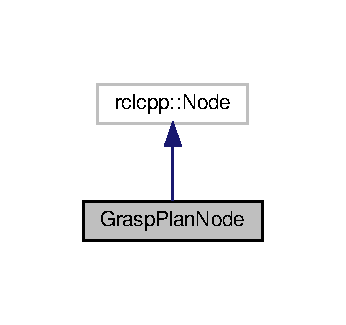
\includegraphics[width=166pt]{classGraspPlanNode__inherit__graph}
\end{center}
\end{figure}


Collaboration diagram for Grasp\+Plan\+Node\+:\nopagebreak
\begin{figure}[H]
\begin{center}
\leavevmode
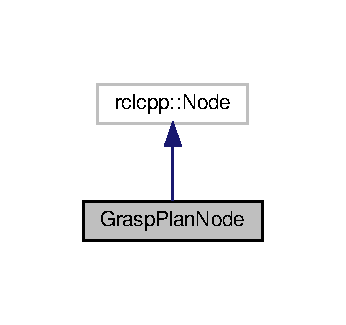
\includegraphics[width=166pt]{classGraspPlanNode__coll__graph}
\end{center}
\end{figure}
\subsection*{Public Attributes}
\begin{DoxyCompactItemize}
\item 
\mbox{\Hypertarget{classGraspPlanNode_a99e4b6352bbd275386e0fe30ad8fd044}\label{classGraspPlanNode_a99e4b6352bbd275386e0fe30ad8fd044}} 
rclcpp\+::\+Publisher$<$ grasp\+\_\+planning\+::msg\+::\+Grasp\+Pose $>$\+::Shared\+Ptr {\bfseries output\+\_\+pub}
\item 
\mbox{\Hypertarget{classGraspPlanNode_a5852a260a5545931888a17b4ee15840e}\label{classGraspPlanNode_a5852a260a5545931888a17b4ee15840e}} 
rclcpp\+::\+Subscription$<$ custom\+\_\+msgs\+::msg\+::\+Rect\+Output $>$\+::Shared\+Ptr {\bfseries perception\+\_\+sub}
\item 
\mbox{\Hypertarget{classGraspPlanNode_acddf7dd4bb3f39ab673a1e380ed2303e}\label{classGraspPlanNode_acddf7dd4bb3f39ab673a1e380ed2303e}} 
boost\+::filesystem\+::path {\bfseries workspace\+\_\+path}
\end{DoxyCompactItemize}


The documentation for this class was generated from the following file\+:\begin{DoxyCompactItemize}
\item 
/home/rosi5/manipulation\+\_\+ws/src/easy\+\_\+manipulation\+\_\+deployment/grasp\+\_\+planner/include/planning\+\_\+node.\+hpp\end{DoxyCompactItemize}

\hypertarget{classMsg}{}\section{Msg Class Reference}
\label{classMsg}\index{Msg@{Msg}}
\subsection*{Public Member Functions}
\begin{DoxyCompactItemize}
\item 
\hyperlink{classMsg_adccb11ca415299593832ae88cf1472b0}{Msg} (const custom\+\_\+msgs\+::msg\+::\+Rect\+Output\+::\+Shared\+Ptr msg, std\+::vector$<$ float $>$ angle\+\_\+)
\end{DoxyCompactItemize}
\subsection*{Public Attributes}
\begin{DoxyCompactItemize}
\item 
\mbox{\Hypertarget{classMsg_af56698dbfa57e8cde6d9fd16ae6eb0c7}\label{classMsg_af56698dbfa57e8cde6d9fd16ae6eb0c7}} 
std\+::vector$<$ float $>$ \hyperlink{classMsg_af56698dbfa57e8cde6d9fd16ae6eb0c7}{bb\+\_\+height}
\begin{DoxyCompactList}\small\item\em Bounding box height. \end{DoxyCompactList}\item 
\mbox{\Hypertarget{classMsg_ab7ce06af06b973cd89e792e4f3ca8f25}\label{classMsg_ab7ce06af06b973cd89e792e4f3ca8f25}} 
std\+::vector$<$ float $>$ \hyperlink{classMsg_ab7ce06af06b973cd89e792e4f3ca8f25}{bb\+\_\+width}
\begin{DoxyCompactList}\small\item\em Bounding box width. \end{DoxyCompactList}\item 
\mbox{\Hypertarget{classMsg_a1a65895dd80d18cae7bc121fab84f620}\label{classMsg_a1a65895dd80d18cae7bc121fab84f620}} 
std\+::vector$<$ float $>$ \hyperlink{classMsg_a1a65895dd80d18cae7bc121fab84f620}{center\+\_\+x}
\begin{DoxyCompactList}\small\item\em Bounding box center (x) \end{DoxyCompactList}\item 
\mbox{\Hypertarget{classMsg_a064310e59c1d085f90c2d8944b4987dc}\label{classMsg_a064310e59c1d085f90c2d8944b4987dc}} 
std\+::vector$<$ float $>$ \hyperlink{classMsg_a064310e59c1d085f90c2d8944b4987dc}{center\+\_\+y}
\begin{DoxyCompactList}\small\item\em Bounding box center (y) \end{DoxyCompactList}\item 
\mbox{\Hypertarget{classMsg_aad984185ad56b7046af1cc39d9117417}\label{classMsg_aad984185ad56b7046af1cc39d9117417}} 
std\+::vector$<$ float $>$ \hyperlink{classMsg_aad984185ad56b7046af1cc39d9117417}{tl\+\_\+x}
\begin{DoxyCompactList}\small\item\em Bounding box Top left corner (x) \end{DoxyCompactList}\item 
\mbox{\Hypertarget{classMsg_aedc56ec506efe2a7bad443c9e8c74500}\label{classMsg_aedc56ec506efe2a7bad443c9e8c74500}} 
std\+::vector$<$ float $>$ \hyperlink{classMsg_aedc56ec506efe2a7bad443c9e8c74500}{tl\+\_\+y}
\begin{DoxyCompactList}\small\item\em Bounding box Top left corner (y) \end{DoxyCompactList}\item 
\mbox{\Hypertarget{classMsg_af35bb671f11882d692ce5e7dc3a2450d}\label{classMsg_af35bb671f11882d692ce5e7dc3a2450d}} 
std\+::vector$<$ float $>$ \hyperlink{classMsg_af35bb671f11882d692ce5e7dc3a2450d}{tr\+\_\+x}
\begin{DoxyCompactList}\small\item\em Bounding box Top right corner (x) \end{DoxyCompactList}\item 
\mbox{\Hypertarget{classMsg_a01a12ff662d24f39f4fd627296856953}\label{classMsg_a01a12ff662d24f39f4fd627296856953}} 
std\+::vector$<$ float $>$ \hyperlink{classMsg_a01a12ff662d24f39f4fd627296856953}{tr\+\_\+y}
\begin{DoxyCompactList}\small\item\em Bounding box Top right corner (y) \end{DoxyCompactList}\item 
\mbox{\Hypertarget{classMsg_a4192f2fd97c9e2cb240f94ea5039f932}\label{classMsg_a4192f2fd97c9e2cb240f94ea5039f932}} 
std\+::vector$<$ float $>$ \hyperlink{classMsg_a4192f2fd97c9e2cb240f94ea5039f932}{br\+\_\+x}
\begin{DoxyCompactList}\small\item\em Bounding box Bottom right corner (x) \end{DoxyCompactList}\item 
\mbox{\Hypertarget{classMsg_a847a86aeb855919ab8cb93e3181ae89a}\label{classMsg_a847a86aeb855919ab8cb93e3181ae89a}} 
std\+::vector$<$ float $>$ \hyperlink{classMsg_a847a86aeb855919ab8cb93e3181ae89a}{br\+\_\+y}
\begin{DoxyCompactList}\small\item\em Bounding box Bottom right corner (y) \end{DoxyCompactList}\item 
\mbox{\Hypertarget{classMsg_a07cba099f9b2d25453153874e2798d77}\label{classMsg_a07cba099f9b2d25453153874e2798d77}} 
std\+::vector$<$ float $>$ \hyperlink{classMsg_a07cba099f9b2d25453153874e2798d77}{bl\+\_\+x}
\begin{DoxyCompactList}\small\item\em Bounding box Bottom left corner (x) \end{DoxyCompactList}\item 
\mbox{\Hypertarget{classMsg_a58c75ea7de8f441e0054384b3be240be}\label{classMsg_a58c75ea7de8f441e0054384b3be240be}} 
std\+::vector$<$ float $>$ \hyperlink{classMsg_a58c75ea7de8f441e0054384b3be240be}{bl\+\_\+y}
\begin{DoxyCompactList}\small\item\em Bounding box Bottom left corner (y) \end{DoxyCompactList}\item 
\mbox{\Hypertarget{classMsg_a227bf9a23dd1cfe4ba4fa4ce4bc87dd0}\label{classMsg_a227bf9a23dd1cfe4ba4fa4ce4bc87dd0}} 
std\+::vector$<$ float $>$ \hyperlink{classMsg_a227bf9a23dd1cfe4ba4fa4ce4bc87dd0}{angle}
\begin{DoxyCompactList}\small\item\em Angle of the O\+B\+J\+E\+CT wrt horizontal image plane. \end{DoxyCompactList}\item 
\mbox{\Hypertarget{classMsg_a9a8786632db452e94da643b3289226ad}\label{classMsg_a9a8786632db452e94da643b3289226ad}} 
float \hyperlink{classMsg_a9a8786632db452e94da643b3289226ad}{img\+\_\+width}
\begin{DoxyCompactList}\small\item\em Image width in pixels. \end{DoxyCompactList}\item 
\mbox{\Hypertarget{classMsg_af095e04f7257b4246c56276925fc5b35}\label{classMsg_af095e04f7257b4246c56276925fc5b35}} 
float \hyperlink{classMsg_af095e04f7257b4246c56276925fc5b35}{img\+\_\+height}
\begin{DoxyCompactList}\small\item\em Image width in pixels. \end{DoxyCompactList}\item 
\mbox{\Hypertarget{classMsg_ac0ca8cef6654423a02d602b8bcc8ccad}\label{classMsg_ac0ca8cef6654423a02d602b8bcc8ccad}} 
int \hyperlink{classMsg_ac0ca8cef6654423a02d602b8bcc8ccad}{num\+\_\+objects}
\begin{DoxyCompactList}\small\item\em Number of objects. \end{DoxyCompactList}\end{DoxyCompactItemize}


\subsection{Constructor \& Destructor Documentation}
\mbox{\Hypertarget{classMsg_adccb11ca415299593832ae88cf1472b0}\label{classMsg_adccb11ca415299593832ae88cf1472b0}} 
\index{Msg@{Msg}!Msg@{Msg}}
\index{Msg@{Msg}!Msg@{Msg}}
\subsubsection{\texorpdfstring{Msg()}{Msg()}}
{\footnotesize\ttfamily Msg\+::\+Msg (\begin{DoxyParamCaption}\item[{const custom\+\_\+msgs\+::msg\+::\+Rect\+Output\+::\+Shared\+Ptr}]{msg,  }\item[{std\+::vector$<$ float $>$}]{angle\+\_\+ }\end{DoxyParamCaption})\hspace{0.3cm}{\ttfamily [inline]}}

Class constructor taking in percpeption message type 

The documentation for this class was generated from the following file\+:\begin{DoxyCompactItemize}
\item 
/home/rosi5/manipulation\+\_\+ws/src/easy\+\_\+manipulation\+\_\+deployment/grasp\+\_\+planner/include/msg.\+hpp\end{DoxyCompactItemize}

\hypertarget{classSuctionCupArray}{}\section{Suction\+Cup\+Array Class Reference}
\label{classSuctionCupArray}\index{Suction\+Cup\+Array@{Suction\+Cup\+Array}}
\subsection*{Public Member Functions}
\begin{DoxyCompactItemize}
\item 
\hyperlink{classSuctionCupArray_a33bbdfb41d4a5b5de459187ee800d317}{Suction\+Cup\+Array} ()
\item 
\hyperlink{classSuctionCupArray_adc7c28d5922124c15c8b31b4ac391879}{Suction\+Cup\+Array} (int length\+\_\+cup\+\_\+num\+\_\+, int breadth\+\_\+cup\+\_\+num\+\_\+, float radius\+\_\+, float table\+\_\+height\+\_\+)
\item 
int \hyperlink{classSuctionCupArray_ae7cb79c848f3067b11cfc98751e143a4}{get\+\_\+cup\+\_\+gdi} (\hyperlink{classMsg}{Msg} msg, cv\+::\+Mat depth\+\_\+img, std\+::vector$<$ int $>$ point, int item\+\_\+num)
\item 
bool \hyperlink{classSuctionCupArray_a342e3be05d1d154a6d7ae1c3564db2d5}{get\+\_\+best\+\_\+grasp} (\hyperlink{classMsg}{Msg} msg, cv\+::\+Mat depth\+\_\+img, int item)
\end{DoxyCompactItemize}
\subsection*{Public Attributes}
\begin{DoxyCompactItemize}
\item 
\mbox{\Hypertarget{classSuctionCupArray_a29d5e8498457d0fa5039444e66d1d178}\label{classSuctionCupArray_a29d5e8498457d0fa5039444e66d1d178}} 
int \hyperlink{classSuctionCupArray_a29d5e8498457d0fa5039444e66d1d178}{length\+\_\+cup\+\_\+num}
\begin{DoxyCompactList}\small\item\em number of suction cups in the length dimension \end{DoxyCompactList}\item 
\mbox{\Hypertarget{classSuctionCupArray_a98d7e70982afefdf3b1eaefc785dda49}\label{classSuctionCupArray_a98d7e70982afefdf3b1eaefc785dda49}} 
int \hyperlink{classSuctionCupArray_a98d7e70982afefdf3b1eaefc785dda49}{breadth\+\_\+cup\+\_\+num}
\begin{DoxyCompactList}\small\item\em number of suction cups in the lbreadth dimension \end{DoxyCompactList}\item 
\mbox{\Hypertarget{classSuctionCupArray_a245c78c0bc387eef40fea1ecab401531}\label{classSuctionCupArray_a245c78c0bc387eef40fea1ecab401531}} 
float \hyperlink{classSuctionCupArray_a245c78c0bc387eef40fea1ecab401531}{radius}
\begin{DoxyCompactList}\small\item\em Radius of each suction cup. \end{DoxyCompactList}\item 
\mbox{\Hypertarget{classSuctionCupArray_a7cd14259831ee3c35bc5dd60c6720afb}\label{classSuctionCupArray_a7cd14259831ee3c35bc5dd60c6720afb}} 
float \hyperlink{classSuctionCupArray_a7cd14259831ee3c35bc5dd60c6720afb}{cup\+\_\+area}
\begin{DoxyCompactList}\small\item\em Area of each suction cup. \end{DoxyCompactList}\item 
\mbox{\Hypertarget{classSuctionCupArray_a95010ae8b7309aea1428b02ff1897d42}\label{classSuctionCupArray_a95010ae8b7309aea1428b02ff1897d42}} 
float \hyperlink{classSuctionCupArray_a95010ae8b7309aea1428b02ff1897d42}{array\+\_\+area}
\begin{DoxyCompactList}\small\item\em Total area the suction cup array covers. \end{DoxyCompactList}\item 
\mbox{\Hypertarget{classSuctionCupArray_a52078f120d8a964f00870e49253a5630}\label{classSuctionCupArray_a52078f120d8a964f00870e49253a5630}} 
float \hyperlink{classSuctionCupArray_a52078f120d8a964f00870e49253a5630}{table\+\_\+height}
\begin{DoxyCompactList}\small\item\em Table height in mm. \end{DoxyCompactList}\item 
\mbox{\Hypertarget{classSuctionCupArray_aa9aedb708c91f8cccd83cdcf09437a44}\label{classSuctionCupArray_aa9aedb708c91f8cccd83cdcf09437a44}} 
float \hyperlink{classSuctionCupArray_aa9aedb708c91f8cccd83cdcf09437a44}{total\+\_\+length}
\begin{DoxyCompactList}\small\item\em Total length of array. \end{DoxyCompactList}\item 
\mbox{\Hypertarget{classSuctionCupArray_aa824e15826e6aa1f860475daec41e17e}\label{classSuctionCupArray_aa824e15826e6aa1f860475daec41e17e}} 
float \hyperlink{classSuctionCupArray_aa824e15826e6aa1f860475daec41e17e}{total\+\_\+breadth}
\begin{DoxyCompactList}\small\item\em Total breadth of array. \end{DoxyCompactList}\item 
\mbox{\Hypertarget{classSuctionCupArray_abc9fedf81d8e05ce102a65773e070255}\label{classSuctionCupArray_abc9fedf81d8e05ce102a65773e070255}} 
float \hyperlink{classSuctionCupArray_abc9fedf81d8e05ce102a65773e070255}{breadth\+\_\+gap} = 0
\begin{DoxyCompactList}\small\item\em length of gap between a the suction cups of an array in the length dimension \end{DoxyCompactList}\item 
\mbox{\Hypertarget{classSuctionCupArray_ad76a4968df08cd66ab4d3673869d7ee6}\label{classSuctionCupArray_ad76a4968df08cd66ab4d3673869d7ee6}} 
float \hyperlink{classSuctionCupArray_ad76a4968df08cd66ab4d3673869d7ee6}{length\+\_\+\+\_\+gap} = 0
\begin{DoxyCompactList}\small\item\em length of gap between a the suction cups of an array in the breadth dimension \end{DoxyCompactList}\item 
\mbox{\Hypertarget{classSuctionCupArray_ada1374d63871766ab0bd82306443b87c}\label{classSuctionCupArray_ada1374d63871766ab0bd82306443b87c}} 
std\+::vector$<$ int $>$ \hyperlink{classSuctionCupArray_ada1374d63871766ab0bd82306443b87c}{chosen\+\_\+grasp}
\begin{DoxyCompactList}\small\item\em Coordinates of the chosen grasp. \end{DoxyCompactList}\item 
\mbox{\Hypertarget{classSuctionCupArray_a6d938bb2d8424798495f1a74ec59300d}\label{classSuctionCupArray_a6d938bb2d8424798495f1a74ec59300d}} 
int \hyperlink{classSuctionCupArray_a6d938bb2d8424798495f1a74ec59300d}{gdi}
\begin{DoxyCompactList}\small\item\em Grasp. \end{DoxyCompactList}\end{DoxyCompactItemize}


\subsection{Constructor \& Destructor Documentation}
\mbox{\Hypertarget{classSuctionCupArray_a33bbdfb41d4a5b5de459187ee800d317}\label{classSuctionCupArray_a33bbdfb41d4a5b5de459187ee800d317}} 
\index{Suction\+Cup\+Array@{Suction\+Cup\+Array}!Suction\+Cup\+Array@{Suction\+Cup\+Array}}
\index{Suction\+Cup\+Array@{Suction\+Cup\+Array}!Suction\+Cup\+Array@{Suction\+Cup\+Array}}
\subsubsection{\texorpdfstring{Suction\+Cup\+Array()}{SuctionCupArray()}\hspace{0.1cm}{\footnotesize\ttfamily [1/2]}}
{\footnotesize\ttfamily Suction\+Cup\+Array\+::\+Suction\+Cup\+Array (\begin{DoxyParamCaption}{ }\end{DoxyParamCaption})\hspace{0.3cm}{\ttfamily [inline]}}

Empty Suction cup array constructor \mbox{\Hypertarget{classSuctionCupArray_adc7c28d5922124c15c8b31b4ac391879}\label{classSuctionCupArray_adc7c28d5922124c15c8b31b4ac391879}} 
\index{Suction\+Cup\+Array@{Suction\+Cup\+Array}!Suction\+Cup\+Array@{Suction\+Cup\+Array}}
\index{Suction\+Cup\+Array@{Suction\+Cup\+Array}!Suction\+Cup\+Array@{Suction\+Cup\+Array}}
\subsubsection{\texorpdfstring{Suction\+Cup\+Array()}{SuctionCupArray()}\hspace{0.1cm}{\footnotesize\ttfamily [2/2]}}
{\footnotesize\ttfamily Suction\+Cup\+Array\+::\+Suction\+Cup\+Array (\begin{DoxyParamCaption}\item[{int}]{length\+\_\+cup\+\_\+num\+\_\+,  }\item[{int}]{breadth\+\_\+cup\+\_\+num\+\_\+,  }\item[{float}]{radius\+\_\+,  }\item[{float}]{table\+\_\+height\+\_\+ }\end{DoxyParamCaption})\hspace{0.3cm}{\ttfamily [inline]}}

Suction cup array constructor 

\subsection{Member Function Documentation}
\mbox{\Hypertarget{classSuctionCupArray_a342e3be05d1d154a6d7ae1c3564db2d5}\label{classSuctionCupArray_a342e3be05d1d154a6d7ae1c3564db2d5}} 
\index{Suction\+Cup\+Array@{Suction\+Cup\+Array}!get\+\_\+best\+\_\+grasp@{get\+\_\+best\+\_\+grasp}}
\index{get\+\_\+best\+\_\+grasp@{get\+\_\+best\+\_\+grasp}!Suction\+Cup\+Array@{Suction\+Cup\+Array}}
\subsubsection{\texorpdfstring{get\+\_\+best\+\_\+grasp()}{get\_best\_grasp()}}
{\footnotesize\ttfamily bool Suction\+Cup\+Array\+::get\+\_\+best\+\_\+grasp (\begin{DoxyParamCaption}\item[{\hyperlink{classMsg}{Msg}}]{msg,  }\item[{cv\+::\+Mat}]{depth\+\_\+img,  }\item[{int}]{item }\end{DoxyParamCaption})\hspace{0.3cm}{\ttfamily [inline]}}

Get the coordinates of the best grasp for the suction cup array \mbox{\Hypertarget{classSuctionCupArray_ae7cb79c848f3067b11cfc98751e143a4}\label{classSuctionCupArray_ae7cb79c848f3067b11cfc98751e143a4}} 
\index{Suction\+Cup\+Array@{Suction\+Cup\+Array}!get\+\_\+cup\+\_\+gdi@{get\+\_\+cup\+\_\+gdi}}
\index{get\+\_\+cup\+\_\+gdi@{get\+\_\+cup\+\_\+gdi}!Suction\+Cup\+Array@{Suction\+Cup\+Array}}
\subsubsection{\texorpdfstring{get\+\_\+cup\+\_\+gdi()}{get\_cup\_gdi()}}
{\footnotesize\ttfamily int Suction\+Cup\+Array\+::get\+\_\+cup\+\_\+gdi (\begin{DoxyParamCaption}\item[{\hyperlink{classMsg}{Msg}}]{msg,  }\item[{cv\+::\+Mat}]{depth\+\_\+img,  }\item[{std\+::vector$<$ int $>$}]{point,  }\item[{int}]{item\+\_\+num }\end{DoxyParamCaption})\hspace{0.3cm}{\ttfamily [inline]}}

Get the Grasp Decide Index of a single suction cup in a suction cup array 

The documentation for this class was generated from the following file\+:\begin{DoxyCompactItemize}
\item 
/home/rosi5/manipulation\+\_\+ws/src/easy\+\_\+manipulation\+\_\+deployment/grasp\+\_\+planner/include/grasps.\+hpp\end{DoxyCompactItemize}

\hypertarget{classTwoFinger}{}\section{Two\+Finger Class Reference}
\label{classTwoFinger}\index{Two\+Finger@{Two\+Finger}}
\subsection*{Public Member Functions}
\begin{DoxyCompactItemize}
\item 
\hyperlink{classTwoFinger_a17e7b3ee5b7e21d99b99968c9c14ac87}{Two\+Finger} ()
\item 
\hyperlink{classTwoFinger_ab0708e05d9ebf755745c14293cf6ddca}{Two\+Finger} (float g\+\_\+thickness, float table\+\_\+height\+\_\+, float distance, float min\+\_\+zero\+\_\+angle\+\_\+, float min\+\_\+height\+\_\+diff\+\_\+to\+\_\+grip\+\_\+, float min\+\_\+gdi\+\_\+diff\+\_\+for\+\_\+comparison\+\_\+)
\item 
void \hyperlink{classTwoFinger_a36ecc602dc5e27c172e62b71ed5d2577}{get\+\_\+checkpoints} (\hyperlink{classMsg}{Msg} msg)
\item 
int \hyperlink{classTwoFinger_a364371baead95faf819ba910fa60e9fd}{get\+\_\+corner\+\_\+gdi} (std\+::vector$<$ int $>$ \hyperlink{classTwoFinger_a2a3e8cfa8504784fcfdcf782deeb6864}{centre}, float radius, cv\+::\+Mat depth\+\_\+img, float centre\+\_\+depth)
\item 
int \hyperlink{classTwoFinger_a9f629646c344238a7b45c68a8f92e179}{get\+\_\+gdi\+\_\+value} (cv\+::\+Mat depth\+\_\+img, std\+::vector$<$ int $>$ target\+\_\+centre, std\+::vector$<$ int $>$ target\+\_\+corner1, std\+::vector$<$ int $>$ target\+\_\+corner2, std\+::vector$<$ int $>$ target\+\_\+corner3, std\+::vector$<$ int $>$ target\+\_\+corner4)
\item 
vector$<$ vector$<$ int $>$ $>$ \hyperlink{classTwoFinger_aaa139685eb927fad02edc52afde35a23}{find\+\_\+2\+\_\+points} (std\+::vector$<$ float $>$ potential\+\_\+corner1, std\+::vector$<$ float $>$potential\+\_\+corner2, int item\+\_\+num)
\item 
int \hyperlink{classTwoFinger_a80d8942ee06dde64fdb4d8928903b4f2}{best\+\_\+grasp\+\_\+from\+\_\+point} (std\+::vector$<$ int $>$ point, \hyperlink{classMsg}{Msg} msg, cv\+::\+Mat depth\+\_\+values, int item\+\_\+num, int curr\+\_\+max\+\_\+gdi)
\item 
bool \hyperlink{classTwoFinger_a4d2eda71d6d313d4b775636d45db1685}{get\+\_\+best\+\_\+grasp} (\hyperlink{classMsg}{Msg} msg, cv\+::\+Mat depth\+\_\+values, int item\+\_\+num)
\end{DoxyCompactItemize}
\subsection*{Public Attributes}
\begin{DoxyCompactItemize}
\item 
\mbox{\Hypertarget{classTwoFinger_a9e74a374c5214aec993bf4dfe856c93c}\label{classTwoFinger_a9e74a374c5214aec993bf4dfe856c93c}} 
std\+::vector$<$ int $>$ \hyperlink{classTwoFinger_a9e74a374c5214aec993bf4dfe856c93c}{corner1}
\begin{DoxyCompactList}\small\item\em Corner 1 of the 2 finger grasp rectangle. \end{DoxyCompactList}\item 
\mbox{\Hypertarget{classTwoFinger_a860d34e5fbd57556fe8313e40eefe5f6}\label{classTwoFinger_a860d34e5fbd57556fe8313e40eefe5f6}} 
std\+::vector$<$ int $>$ \hyperlink{classTwoFinger_a860d34e5fbd57556fe8313e40eefe5f6}{corner2}
\begin{DoxyCompactList}\small\item\em Corner 2 of the 2 finger grasp rectangle. \end{DoxyCompactList}\item 
\mbox{\Hypertarget{classTwoFinger_a3ef052222752b0fc0ed4ef951d89b4e1}\label{classTwoFinger_a3ef052222752b0fc0ed4ef951d89b4e1}} 
std\+::vector$<$ int $>$ \hyperlink{classTwoFinger_a3ef052222752b0fc0ed4ef951d89b4e1}{corner3}
\begin{DoxyCompactList}\small\item\em Corner 3 of the 2 finger grasp rectangle. \end{DoxyCompactList}\item 
\mbox{\Hypertarget{classTwoFinger_a88c6337a2c26521c81d849fa4e244256}\label{classTwoFinger_a88c6337a2c26521c81d849fa4e244256}} 
std\+::vector$<$ int $>$ \hyperlink{classTwoFinger_a88c6337a2c26521c81d849fa4e244256}{corner4}
\begin{DoxyCompactList}\small\item\em Corner 4 of the 2 finger grasp rectangle. \end{DoxyCompactList}\item 
\mbox{\Hypertarget{classTwoFinger_ab9eb97029e3fe8e4c9c3e931fde0b652}\label{classTwoFinger_ab9eb97029e3fe8e4c9c3e931fde0b652}} 
int \hyperlink{classTwoFinger_ab9eb97029e3fe8e4c9c3e931fde0b652}{final\+\_\+gdi}
\begin{DoxyCompactList}\small\item\em Final grasp quality of the chosen grasp. \end{DoxyCompactList}\item 
\mbox{\Hypertarget{classTwoFinger_a6fe537b025bf208d56cb1632a1eb5ff0}\label{classTwoFinger_a6fe537b025bf208d56cb1632a1eb5ff0}} 
float \hyperlink{classTwoFinger_a6fe537b025bf208d56cb1632a1eb5ff0}{min\+\_\+zero\+\_\+angle}
\begin{DoxyCompactList}\small\item\em Minimum angle to be considered as zero. Prevents errors from very small angles. \end{DoxyCompactList}\item 
\mbox{\Hypertarget{classTwoFinger_a0630b6d72b7f2acfb730758a7bf3907a}\label{classTwoFinger_a0630b6d72b7f2acfb730758a7bf3907a}} 
float \hyperlink{classTwoFinger_a0630b6d72b7f2acfb730758a7bf3907a}{min\+\_\+height\+\_\+diff\+\_\+to\+\_\+grip}
\begin{DoxyCompactList}\small\item\em in mm. minimum height needed to pinch an object. Determine the limits for corner collisions \end{DoxyCompactList}\item 
\mbox{\Hypertarget{classTwoFinger_aebc0eacece70162a016a2f670a17c811}\label{classTwoFinger_aebc0eacece70162a016a2f670a17c811}} 
float \hyperlink{classTwoFinger_aebc0eacece70162a016a2f670a17c811}{min\+\_\+gdi\+\_\+diff\+\_\+for\+\_\+comparison}
\begin{DoxyCompactList}\small\item\em When Comparing grasp G\+DI, We only want to include centre G\+DI if the grasp G\+DI is similar. This parameter determines how close should a G\+DI be to be considered equal. \end{DoxyCompactList}\item 
\mbox{\Hypertarget{classTwoFinger_a0ef7222d080314043525e634e163cc0a}\label{classTwoFinger_a0ef7222d080314043525e634e163cc0a}} 
int \hyperlink{classTwoFinger_a0ef7222d080314043525e634e163cc0a}{centre\+\_\+gdi\+\_\+max}
\begin{DoxyCompactList}\small\item\em Maximum value of the centre G\+DI. \end{DoxyCompactList}\item 
\mbox{\Hypertarget{classTwoFinger_a568d04dcbb39579810299084850a41a4}\label{classTwoFinger_a568d04dcbb39579810299084850a41a4}} 
int \hyperlink{classTwoFinger_a568d04dcbb39579810299084850a41a4}{potential\+\_\+gdi\+\_\+max}
\begin{DoxyCompactList}\small\item\em Intermediate placeholder for the maximum G\+DI for the current grasp. \end{DoxyCompactList}\item 
\mbox{\Hypertarget{classTwoFinger_a2a3e8cfa8504784fcfdcf782deeb6864}\label{classTwoFinger_a2a3e8cfa8504784fcfdcf782deeb6864}} 
std\+::vector$<$ int $>$ \hyperlink{classTwoFinger_a2a3e8cfa8504784fcfdcf782deeb6864}{centre}
\begin{DoxyCompactList}\small\item\em Centre of grasp rectangle. \end{DoxyCompactList}\item 
\mbox{\Hypertarget{classTwoFinger_a3057c3696a07f03a5a95ecc2abdf16da}\label{classTwoFinger_a3057c3696a07f03a5a95ecc2abdf16da}} 
float \hyperlink{classTwoFinger_a3057c3696a07f03a5a95ecc2abdf16da}{table\+\_\+height}
\begin{DoxyCompactList}\small\item\em Table height in mm. \end{DoxyCompactList}\item 
\mbox{\Hypertarget{classTwoFinger_afb0ad9bb2961d227461190e499aeb16e}\label{classTwoFinger_afb0ad9bb2961d227461190e499aeb16e}} 
float \hyperlink{classTwoFinger_afb0ad9bb2961d227461190e499aeb16e}{distance\+\_\+between\+\_\+fingers}
\begin{DoxyCompactList}\small\item\em Distance between fingers in pixels. \end{DoxyCompactList}\item 
\mbox{\Hypertarget{classTwoFinger_a0f27dc02232404233f2ae78846d063aa}\label{classTwoFinger_a0f27dc02232404233f2ae78846d063aa}} 
float \hyperlink{classTwoFinger_a0f27dc02232404233f2ae78846d063aa}{gripper\+\_\+thickness}
\begin{DoxyCompactList}\small\item\em Gripper finger thickness in pixels. \end{DoxyCompactList}\item 
\mbox{\Hypertarget{classTwoFinger_a476c6f304358edffd0c3e5fec5a15cf3}\label{classTwoFinger_a476c6f304358edffd0c3e5fec5a15cf3}} 
float \hyperlink{classTwoFinger_a476c6f304358edffd0c3e5fec5a15cf3}{target\+\_\+length}
\begin{DoxyCompactList}\small\item\em Target hypotenuse length of a grasp rectangle. \end{DoxyCompactList}\item 
float \hyperlink{classTwoFinger_a180e995cc0516a1664f88e9067ff0ae0}{allowable\+\_\+length\+\_\+error}
\begin{DoxyCompactList}\small\item\em As the diagonal length of a 2 finger gripper is constant, the length between the two points should be equal to that length We give a certain allowable error of the length between 2 chosen points. \end{DoxyCompactList}\item 
\mbox{\Hypertarget{classTwoFinger_aecf45fe9ca431e9cb3e2844686b112f3}\label{classTwoFinger_aecf45fe9ca431e9cb3e2844686b112f3}} 
std\+::vector$<$ std\+::vector$<$ int $>$ $>$ \hyperlink{classTwoFinger_aecf45fe9ca431e9cb3e2844686b112f3}{checkpoint\+\_\+startx}
\begin{DoxyCompactList}\small\item\em Start x coordinates of grasp sampling. \end{DoxyCompactList}\item 
\mbox{\Hypertarget{classTwoFinger_afb2bad19c2dfabb035af09e5c96fabf3}\label{classTwoFinger_afb2bad19c2dfabb035af09e5c96fabf3}} 
std\+::vector$<$ std\+::vector$<$ int $>$ $>$ \hyperlink{classTwoFinger_afb2bad19c2dfabb035af09e5c96fabf3}{checkpoint\+\_\+starty}
\begin{DoxyCompactList}\small\item\em Start y coordinates of grasp sampling. \end{DoxyCompactList}\item 
\mbox{\Hypertarget{classTwoFinger_afaf5faa229c2a95f0233a180643a905d}\label{classTwoFinger_afaf5faa229c2a95f0233a180643a905d}} 
std\+::vector$<$ std\+::vector$<$ int $>$ $>$ \hyperlink{classTwoFinger_afaf5faa229c2a95f0233a180643a905d}{checkpoint\+\_\+endx}
\begin{DoxyCompactList}\small\item\em End x coordinates of grasp sampling. \end{DoxyCompactList}\item 
\mbox{\Hypertarget{classTwoFinger_aa4b0f0761ef17a83edf7548c57ddbe06}\label{classTwoFinger_aa4b0f0761ef17a83edf7548c57ddbe06}} 
std\+::vector$<$ std\+::vector$<$ int $>$ $>$ \hyperlink{classTwoFinger_aa4b0f0761ef17a83edf7548c57ddbe06}{checkpoint\+\_\+endy}
\begin{DoxyCompactList}\small\item\em End y coordinates of grasp\+\_\+sampling. \end{DoxyCompactList}\item 
\mbox{\Hypertarget{classTwoFinger_a703a859bf7ac397ef7a00f85d540d873}\label{classTwoFinger_a703a859bf7ac397ef7a00f85d540d873}} 
std\+::vector$<$ float $>$ \hyperlink{classTwoFinger_a703a859bf7ac397ef7a00f85d540d873}{gradient\+\_\+vector}
\begin{DoxyCompactList}\small\item\em y-\/intersect vector of the gradient of the 2 lines that represents the bounds of the grasp samples for all objects \end{DoxyCompactList}\item 
\mbox{\Hypertarget{classTwoFinger_a5ed3318155737fe2f9cd07118864595f}\label{classTwoFinger_a5ed3318155737fe2f9cd07118864595f}} 
std\+::vector$<$ float $>$ \hyperlink{classTwoFinger_a5ed3318155737fe2f9cd07118864595f}{c1\+\_\+vector}
\begin{DoxyCompactList}\small\item\em first y-\/intersect vector of the gradient of the 2 lines that represents the bounds of the grasp samples for all objects \end{DoxyCompactList}\item 
\mbox{\Hypertarget{classTwoFinger_afdf53c9910ad01f1b6db85da3ae71cfd}\label{classTwoFinger_afdf53c9910ad01f1b6db85da3ae71cfd}} 
std\+::vector$<$ float $>$ \hyperlink{classTwoFinger_afdf53c9910ad01f1b6db85da3ae71cfd}{c2\+\_\+vector}
\begin{DoxyCompactList}\small\item\em second y-\/intersect vector of the gradient of the 2 lines that represents the bounds of the grasp samples for all objects \end{DoxyCompactList}\end{DoxyCompactItemize}


\subsection{Constructor \& Destructor Documentation}
\mbox{\Hypertarget{classTwoFinger_a17e7b3ee5b7e21d99b99968c9c14ac87}\label{classTwoFinger_a17e7b3ee5b7e21d99b99968c9c14ac87}} 
\index{Two\+Finger@{Two\+Finger}!Two\+Finger@{Two\+Finger}}
\index{Two\+Finger@{Two\+Finger}!Two\+Finger@{Two\+Finger}}
\subsubsection{\texorpdfstring{Two\+Finger()}{TwoFinger()}\hspace{0.1cm}{\footnotesize\ttfamily [1/2]}}
{\footnotesize\ttfamily Two\+Finger\+::\+Two\+Finger (\begin{DoxyParamCaption}{ }\end{DoxyParamCaption})\hspace{0.3cm}{\ttfamily [inline]}}

Constructor for an empty two finger grasp, used usually when there is no grasp \mbox{\Hypertarget{classTwoFinger_ab0708e05d9ebf755745c14293cf6ddca}\label{classTwoFinger_ab0708e05d9ebf755745c14293cf6ddca}} 
\index{Two\+Finger@{Two\+Finger}!Two\+Finger@{Two\+Finger}}
\index{Two\+Finger@{Two\+Finger}!Two\+Finger@{Two\+Finger}}
\subsubsection{\texorpdfstring{Two\+Finger()}{TwoFinger()}\hspace{0.1cm}{\footnotesize\ttfamily [2/2]}}
{\footnotesize\ttfamily Two\+Finger\+::\+Two\+Finger (\begin{DoxyParamCaption}\item[{float}]{g\+\_\+thickness,  }\item[{float}]{table\+\_\+height\+\_\+,  }\item[{float}]{distance,  }\item[{float}]{min\+\_\+zero\+\_\+angle\+\_\+,  }\item[{float}]{min\+\_\+height\+\_\+diff\+\_\+to\+\_\+grip\+\_\+,  }\item[{float}]{min\+\_\+gdi\+\_\+diff\+\_\+for\+\_\+comparison\+\_\+ }\end{DoxyParamCaption})\hspace{0.3cm}{\ttfamily [inline]}}

Constructor for a considered grasp. As the input points represent diagonally opposite points for the grasp rectangle, populate point 1 and 3 

\subsection{Member Function Documentation}
\mbox{\Hypertarget{classTwoFinger_a80d8942ee06dde64fdb4d8928903b4f2}\label{classTwoFinger_a80d8942ee06dde64fdb4d8928903b4f2}} 
\index{Two\+Finger@{Two\+Finger}!best\+\_\+grasp\+\_\+from\+\_\+point@{best\+\_\+grasp\+\_\+from\+\_\+point}}
\index{best\+\_\+grasp\+\_\+from\+\_\+point@{best\+\_\+grasp\+\_\+from\+\_\+point}!Two\+Finger@{Two\+Finger}}
\subsubsection{\texorpdfstring{best\+\_\+grasp\+\_\+from\+\_\+point()}{best\_grasp\_from\_point()}}
{\footnotesize\ttfamily int Two\+Finger\+::best\+\_\+grasp\+\_\+from\+\_\+point (\begin{DoxyParamCaption}\item[{std\+::vector$<$ int $>$}]{point,  }\item[{\hyperlink{classMsg}{Msg}}]{msg,  }\item[{cv\+::\+Mat}]{depth\+\_\+values,  }\item[{int}]{item\+\_\+num,  }\item[{int}]{curr\+\_\+max\+\_\+gdi }\end{DoxyParamCaption})\hspace{0.3cm}{\ttfamily [inline]}}

Samples all possible grasps from a point and chooses the best one \mbox{\Hypertarget{classTwoFinger_aaa139685eb927fad02edc52afde35a23}\label{classTwoFinger_aaa139685eb927fad02edc52afde35a23}} 
\index{Two\+Finger@{Two\+Finger}!find\+\_\+2\+\_\+points@{find\+\_\+2\+\_\+points}}
\index{find\+\_\+2\+\_\+points@{find\+\_\+2\+\_\+points}!Two\+Finger@{Two\+Finger}}
\subsubsection{\texorpdfstring{find\+\_\+2\+\_\+points()}{find\_2\_points()}}
{\footnotesize\ttfamily vector$<$vector$<$int$>$ $>$ Two\+Finger\+::find\+\_\+2\+\_\+points (\begin{DoxyParamCaption}\item[{std\+::vector$<$ float $>$}]{potential\+\_\+corner1,  }\item[{std\+::vector$<$ float $>$}]{potential\+\_\+corner2,  }\item[{int}]{item\+\_\+num }\end{DoxyParamCaption})\hspace{0.3cm}{\ttfamily [inline]}}

Given the coordinates of 2 corners of a grasp, find the coordinates of the other two corners of grasp \mbox{\Hypertarget{classTwoFinger_a4d2eda71d6d313d4b775636d45db1685}\label{classTwoFinger_a4d2eda71d6d313d4b775636d45db1685}} 
\index{Two\+Finger@{Two\+Finger}!get\+\_\+best\+\_\+grasp@{get\+\_\+best\+\_\+grasp}}
\index{get\+\_\+best\+\_\+grasp@{get\+\_\+best\+\_\+grasp}!Two\+Finger@{Two\+Finger}}
\subsubsection{\texorpdfstring{get\+\_\+best\+\_\+grasp()}{get\_best\_grasp()}}
{\footnotesize\ttfamily bool Two\+Finger\+::get\+\_\+best\+\_\+grasp (\begin{DoxyParamCaption}\item[{\hyperlink{classMsg}{Msg}}]{msg,  }\item[{cv\+::\+Mat}]{depth\+\_\+values,  }\item[{int}]{item\+\_\+num }\end{DoxyParamCaption})\hspace{0.3cm}{\ttfamily [inline]}}

Iterate through all points to generate the best possible grasp \mbox{\Hypertarget{classTwoFinger_a36ecc602dc5e27c172e62b71ed5d2577}\label{classTwoFinger_a36ecc602dc5e27c172e62b71ed5d2577}} 
\index{Two\+Finger@{Two\+Finger}!get\+\_\+checkpoints@{get\+\_\+checkpoints}}
\index{get\+\_\+checkpoints@{get\+\_\+checkpoints}!Two\+Finger@{Two\+Finger}}
\subsubsection{\texorpdfstring{get\+\_\+checkpoints()}{get\_checkpoints()}}
{\footnotesize\ttfamily void Two\+Finger\+::get\+\_\+checkpoints (\begin{DoxyParamCaption}\item[{\hyperlink{classMsg}{Msg}}]{msg }\end{DoxyParamCaption})\hspace{0.3cm}{\ttfamily [inline]}}

Get points to be sampled for grasp. The points will be along 2 lines which are reprenting the maximum ends of each side of the 2F gripper \mbox{\Hypertarget{classTwoFinger_a364371baead95faf819ba910fa60e9fd}\label{classTwoFinger_a364371baead95faf819ba910fa60e9fd}} 
\index{Two\+Finger@{Two\+Finger}!get\+\_\+corner\+\_\+gdi@{get\+\_\+corner\+\_\+gdi}}
\index{get\+\_\+corner\+\_\+gdi@{get\+\_\+corner\+\_\+gdi}!Two\+Finger@{Two\+Finger}}
\subsubsection{\texorpdfstring{get\+\_\+corner\+\_\+gdi()}{get\_corner\_gdi()}}
{\footnotesize\ttfamily int Two\+Finger\+::get\+\_\+corner\+\_\+gdi (\begin{DoxyParamCaption}\item[{std\+::vector$<$ int $>$}]{centre,  }\item[{float}]{radius,  }\item[{cv\+::\+Mat}]{depth\+\_\+img,  }\item[{float}]{centre\+\_\+depth }\end{DoxyParamCaption})\hspace{0.3cm}{\ttfamily [inline]}}

Calculating the grasp quality of one side of a grasp rectangle \mbox{\Hypertarget{classTwoFinger_a9f629646c344238a7b45c68a8f92e179}\label{classTwoFinger_a9f629646c344238a7b45c68a8f92e179}} 
\index{Two\+Finger@{Two\+Finger}!get\+\_\+gdi\+\_\+value@{get\+\_\+gdi\+\_\+value}}
\index{get\+\_\+gdi\+\_\+value@{get\+\_\+gdi\+\_\+value}!Two\+Finger@{Two\+Finger}}
\subsubsection{\texorpdfstring{get\+\_\+gdi\+\_\+value()}{get\_gdi\_value()}}
{\footnotesize\ttfamily int Two\+Finger\+::get\+\_\+gdi\+\_\+value (\begin{DoxyParamCaption}\item[{cv\+::\+Mat}]{depth\+\_\+img,  }\item[{std\+::vector$<$ int $>$}]{target\+\_\+centre,  }\item[{std\+::vector$<$ int $>$}]{target\+\_\+corner1,  }\item[{std\+::vector$<$ int $>$}]{target\+\_\+corner2,  }\item[{std\+::vector$<$ int $>$}]{target\+\_\+corner3,  }\item[{std\+::vector$<$ int $>$}]{target\+\_\+corner4 }\end{DoxyParamCaption})\hspace{0.3cm}{\ttfamily [inline]}}

Generates a Grasp Decide Index value which measures the quality of a grasp approach. 

\subsection{Member Data Documentation}
\mbox{\Hypertarget{classTwoFinger_a180e995cc0516a1664f88e9067ff0ae0}\label{classTwoFinger_a180e995cc0516a1664f88e9067ff0ae0}} 
\index{Two\+Finger@{Two\+Finger}!allowable\+\_\+length\+\_\+error@{allowable\+\_\+length\+\_\+error}}
\index{allowable\+\_\+length\+\_\+error@{allowable\+\_\+length\+\_\+error}!Two\+Finger@{Two\+Finger}}
\subsubsection{\texorpdfstring{allowable\+\_\+length\+\_\+error}{allowable\_length\_error}}
{\footnotesize\ttfamily float Two\+Finger\+::allowable\+\_\+length\+\_\+error}



As the diagonal length of a 2 finger gripper is constant, the length between the two points should be equal to that length We give a certain allowable error of the length between 2 chosen points. 

T\+O\+DO\+:There needs to be a way to change this depending on orientation. When it is vertical or horizontal, the allowable error should be lower compared to an angled object 

The documentation for this class was generated from the following file\+:\begin{DoxyCompactItemize}
\item 
/home/rosi5/manipulation\+\_\+ws/src/easy\+\_\+manipulation\+\_\+deployment/grasp\+\_\+planner/include/grasps.\+hpp\end{DoxyCompactItemize}

%--- End generated contents ---

% Index
\backmatter
\newpage
\phantomsection
\clearemptydoublepage
\addcontentsline{toc}{chapter}{Index}
\printindex

\end{document}
